\begin{prob}
    The code below is a modified version of BFS shown in class. This
    modification has a single addition: a \python{print} statement. A comment
    in the code indicates where the \python{print} statement is located.

    \begin{minted}[autogobble]{python}
        def bfs(graph, source):
            """Start a BFS at `source`."""
            status = {node: 'undiscovered' for node in graph.nodes}
            status[source] = 'pending'
            pending = deque([source])

            while pending: 
                u = pending.popleft()
                for v in graph.neighbors(u):
                    print("here!") # <--- this is the print statement
                    if status[v] == 'undiscovered':
                        status[v] = 'pending'
                        pending.append(v)
                status[u] = 'visited'
    \end{minted}

    Suppose this modified BFS is run on the following graph, starting at node
    $a$.

    \begin{center} 
        
    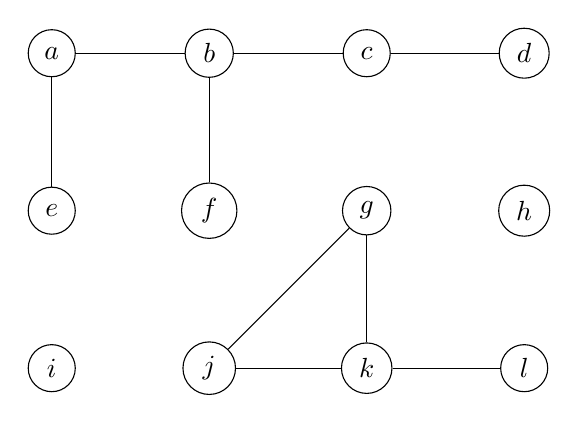
\begin{tikzpicture}
        \tikzset{every node/.style = {shape=circle, draw, minimum size=17pt}}

        \node (a) at (0, 0) {$a$};
        \node (b) at (2, 0) {$b$};
        \node (c) at (4, 0) {$c$};
        \node (d) at (6, 0) {$d$};

        \node (e) at (0, -2) {$e$};
        \node (f) at (2, -2) {$f$};
        \node (g) at (4, -2) {$g$};
        \node (h) at (6, -2) {$h$};

        \node (i) at (0, -4) {$i$};
        \node (j) at (2, -4) {$j$};
        \node (k) at (4, -4) {$k$};
        \node (l) at (6, -4) {$l$};

        \draw (a) edge (b);
        \draw (b) edge (c);
        \draw (c) edge (d);

        \draw (a) edge (e);
        \draw (b) edge (f);

        \draw (k) edge (l);

        \draw (j) edge (g);
        \draw (k) edge (g);
        \draw (k) edge (j);

    \end{tikzpicture}
    \end{center}

    How many times will \python{"here!"} be printed? Your answer should be an exact number.

    \inlineresponsebox[.75in]{10}

\end{prob}
